\documentclass[conference,compsoc]{IEEEtran}
\usepackage{cite}
\usepackage[english]{babel}
\usepackage[pdftex]{graphicx}
 \usepackage{array}
\usepackage{multirow}
\DeclareGraphicsExtensions{.pdf,.jpeg,.png}
\usepackage{amsmath}
\usepackage[caption=false,font=footnotesize,labelfont=sf,textfont=sf]{subfig}
\usepackage{url}
\hyphenation{op-tical net-works semi-conduc-tor}

\makeatletter
\def\endthebibliography{%
	\def\@noitemerr{\@latex@warning{Empty `thebibliography' environment}}%
	\endlist
}
\makeatother

\begin{document}
\title{Data Driven Project Management \\ Predicting the Development Time}


\author{\IEEEauthorblockN{Marko Prelevikj}
	\IEEEauthorblockA{Faculty of Computer and Information Science\\
		University of Ljubljana\\
		Ljubljana, Slovenia\\
		Email: mp2638@stuent.uni-lj.si}
}

\maketitle

\begin{abstract}
Predicting development time is hard. In this paper we are trying to explain all the difficulties encountered on the journey to predicting time with as low 
\end{abstract}

\IEEEpeerreviewmaketitle

\section{Introduction}
explain PMO's problems
\section{Model data}
JIRA data briefly and what the model is consisted of



\section{Testing model quality}
Present different the results (MAE, RMSE, R2) obtained by different regressors.
As the variance lowers, so do the metrics of quality of the models.
\section{Model Explainability}
Write about feature importance and how to explain the made decisions.


\section{Conclusion}
Quick recap of the problem and how we solved it.
XGBoost~\cite{chen2016xgXGBoost}, SHAP~\cite{lundberg2020local2global}.

\begin{figure}[!t]
\centering
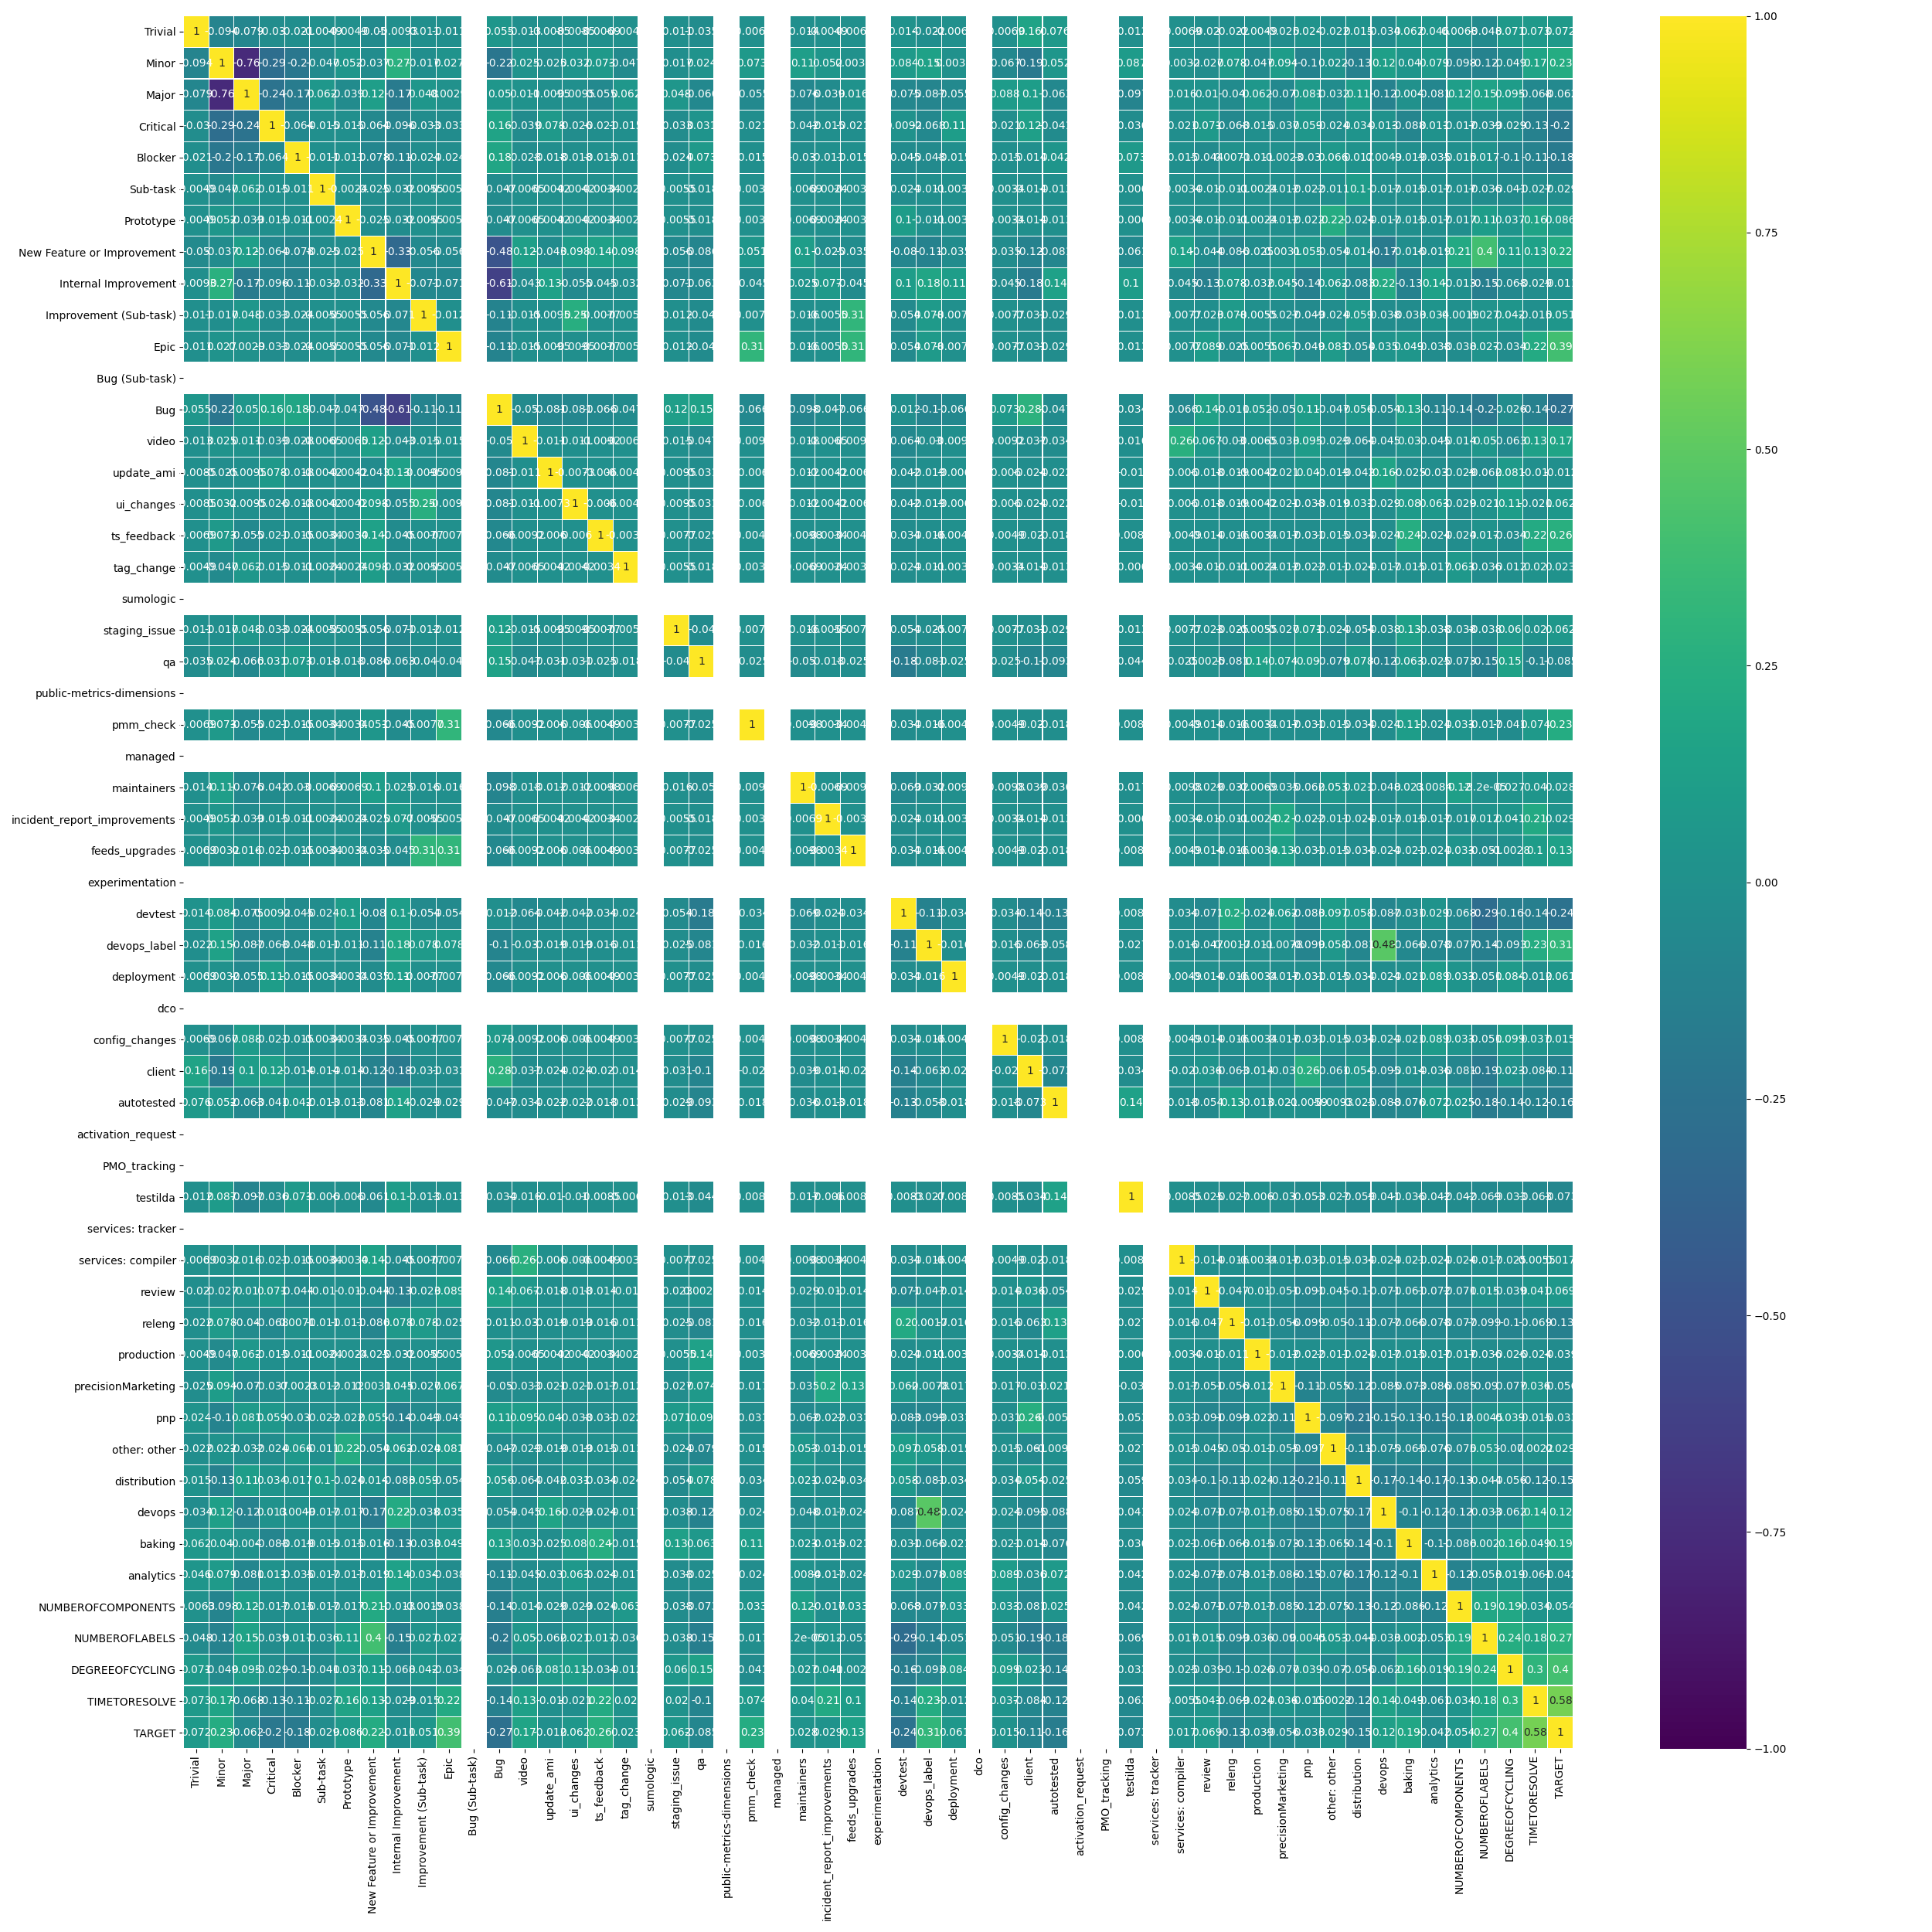
\includegraphics[width=2.5in]{feature_correlation.png}
\caption{Simulation results for the network.}
\label{fig_sim}
\end{figure}

\begin{figure*}[!t]
\centering
\subfloat[Case I]{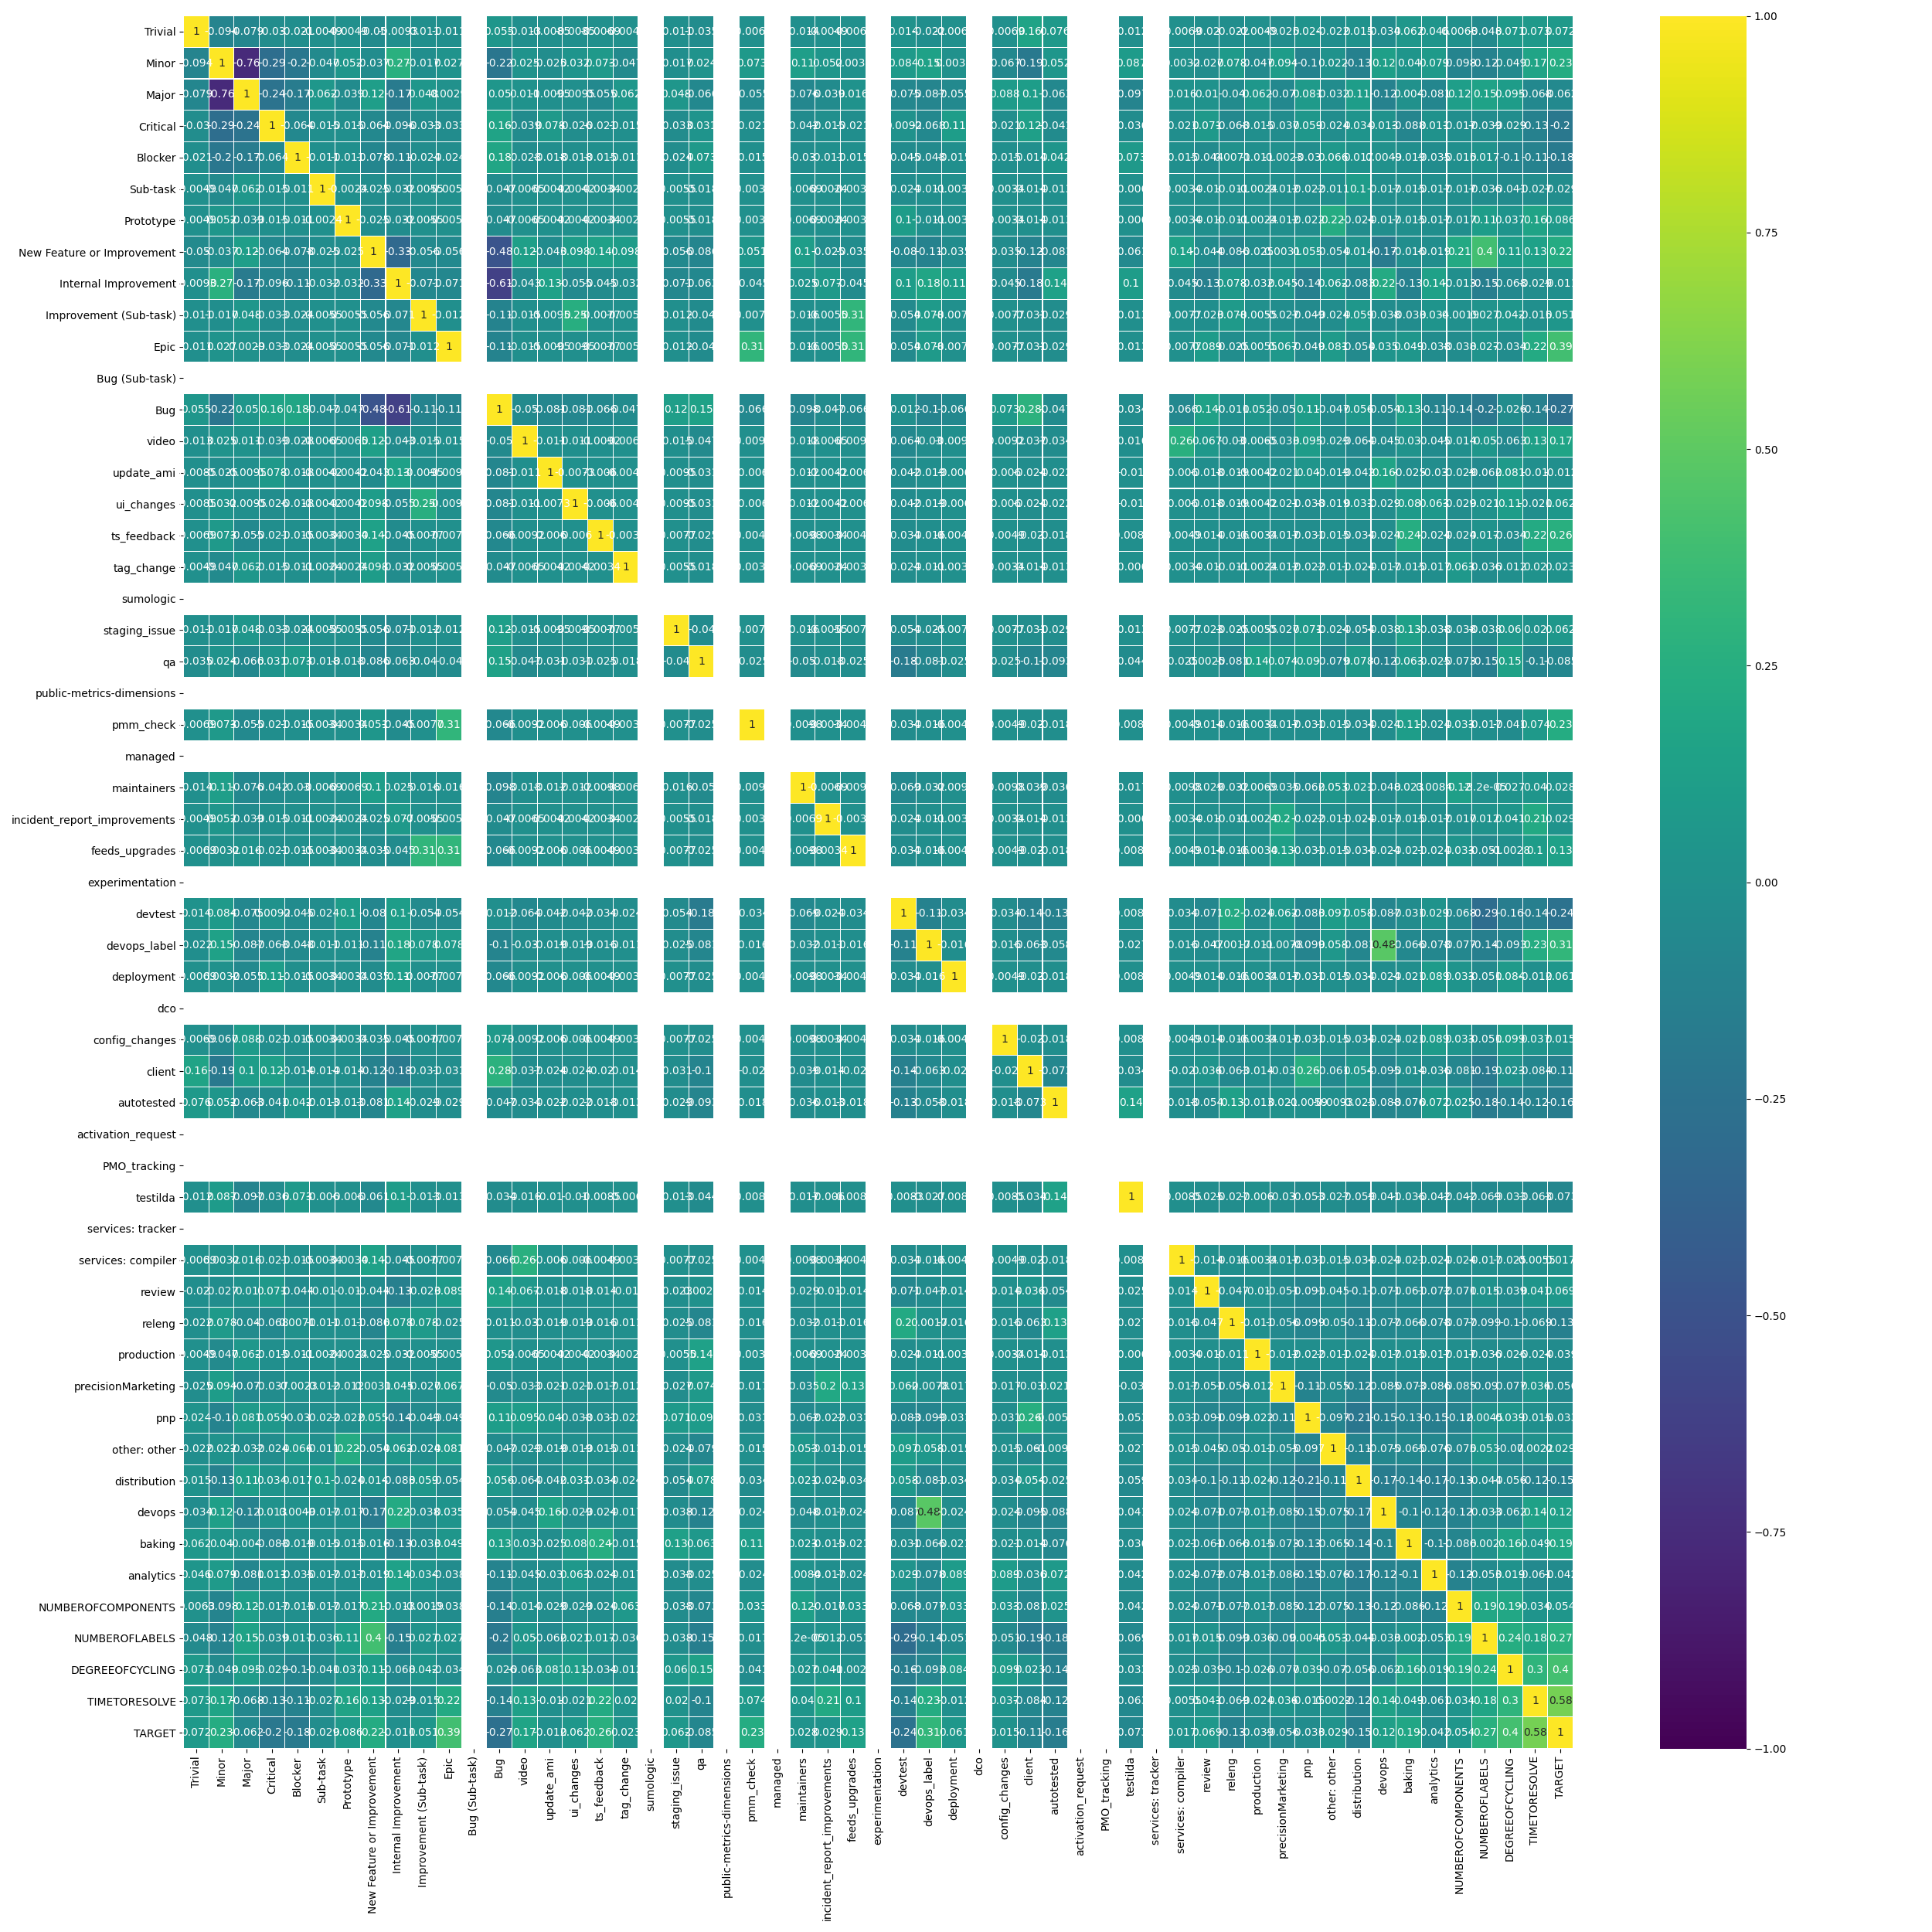
\includegraphics[width=2.5in]{feature_correlation.png}%
\label{fig_first_case}}
\hfil
\subfloat[Case II]{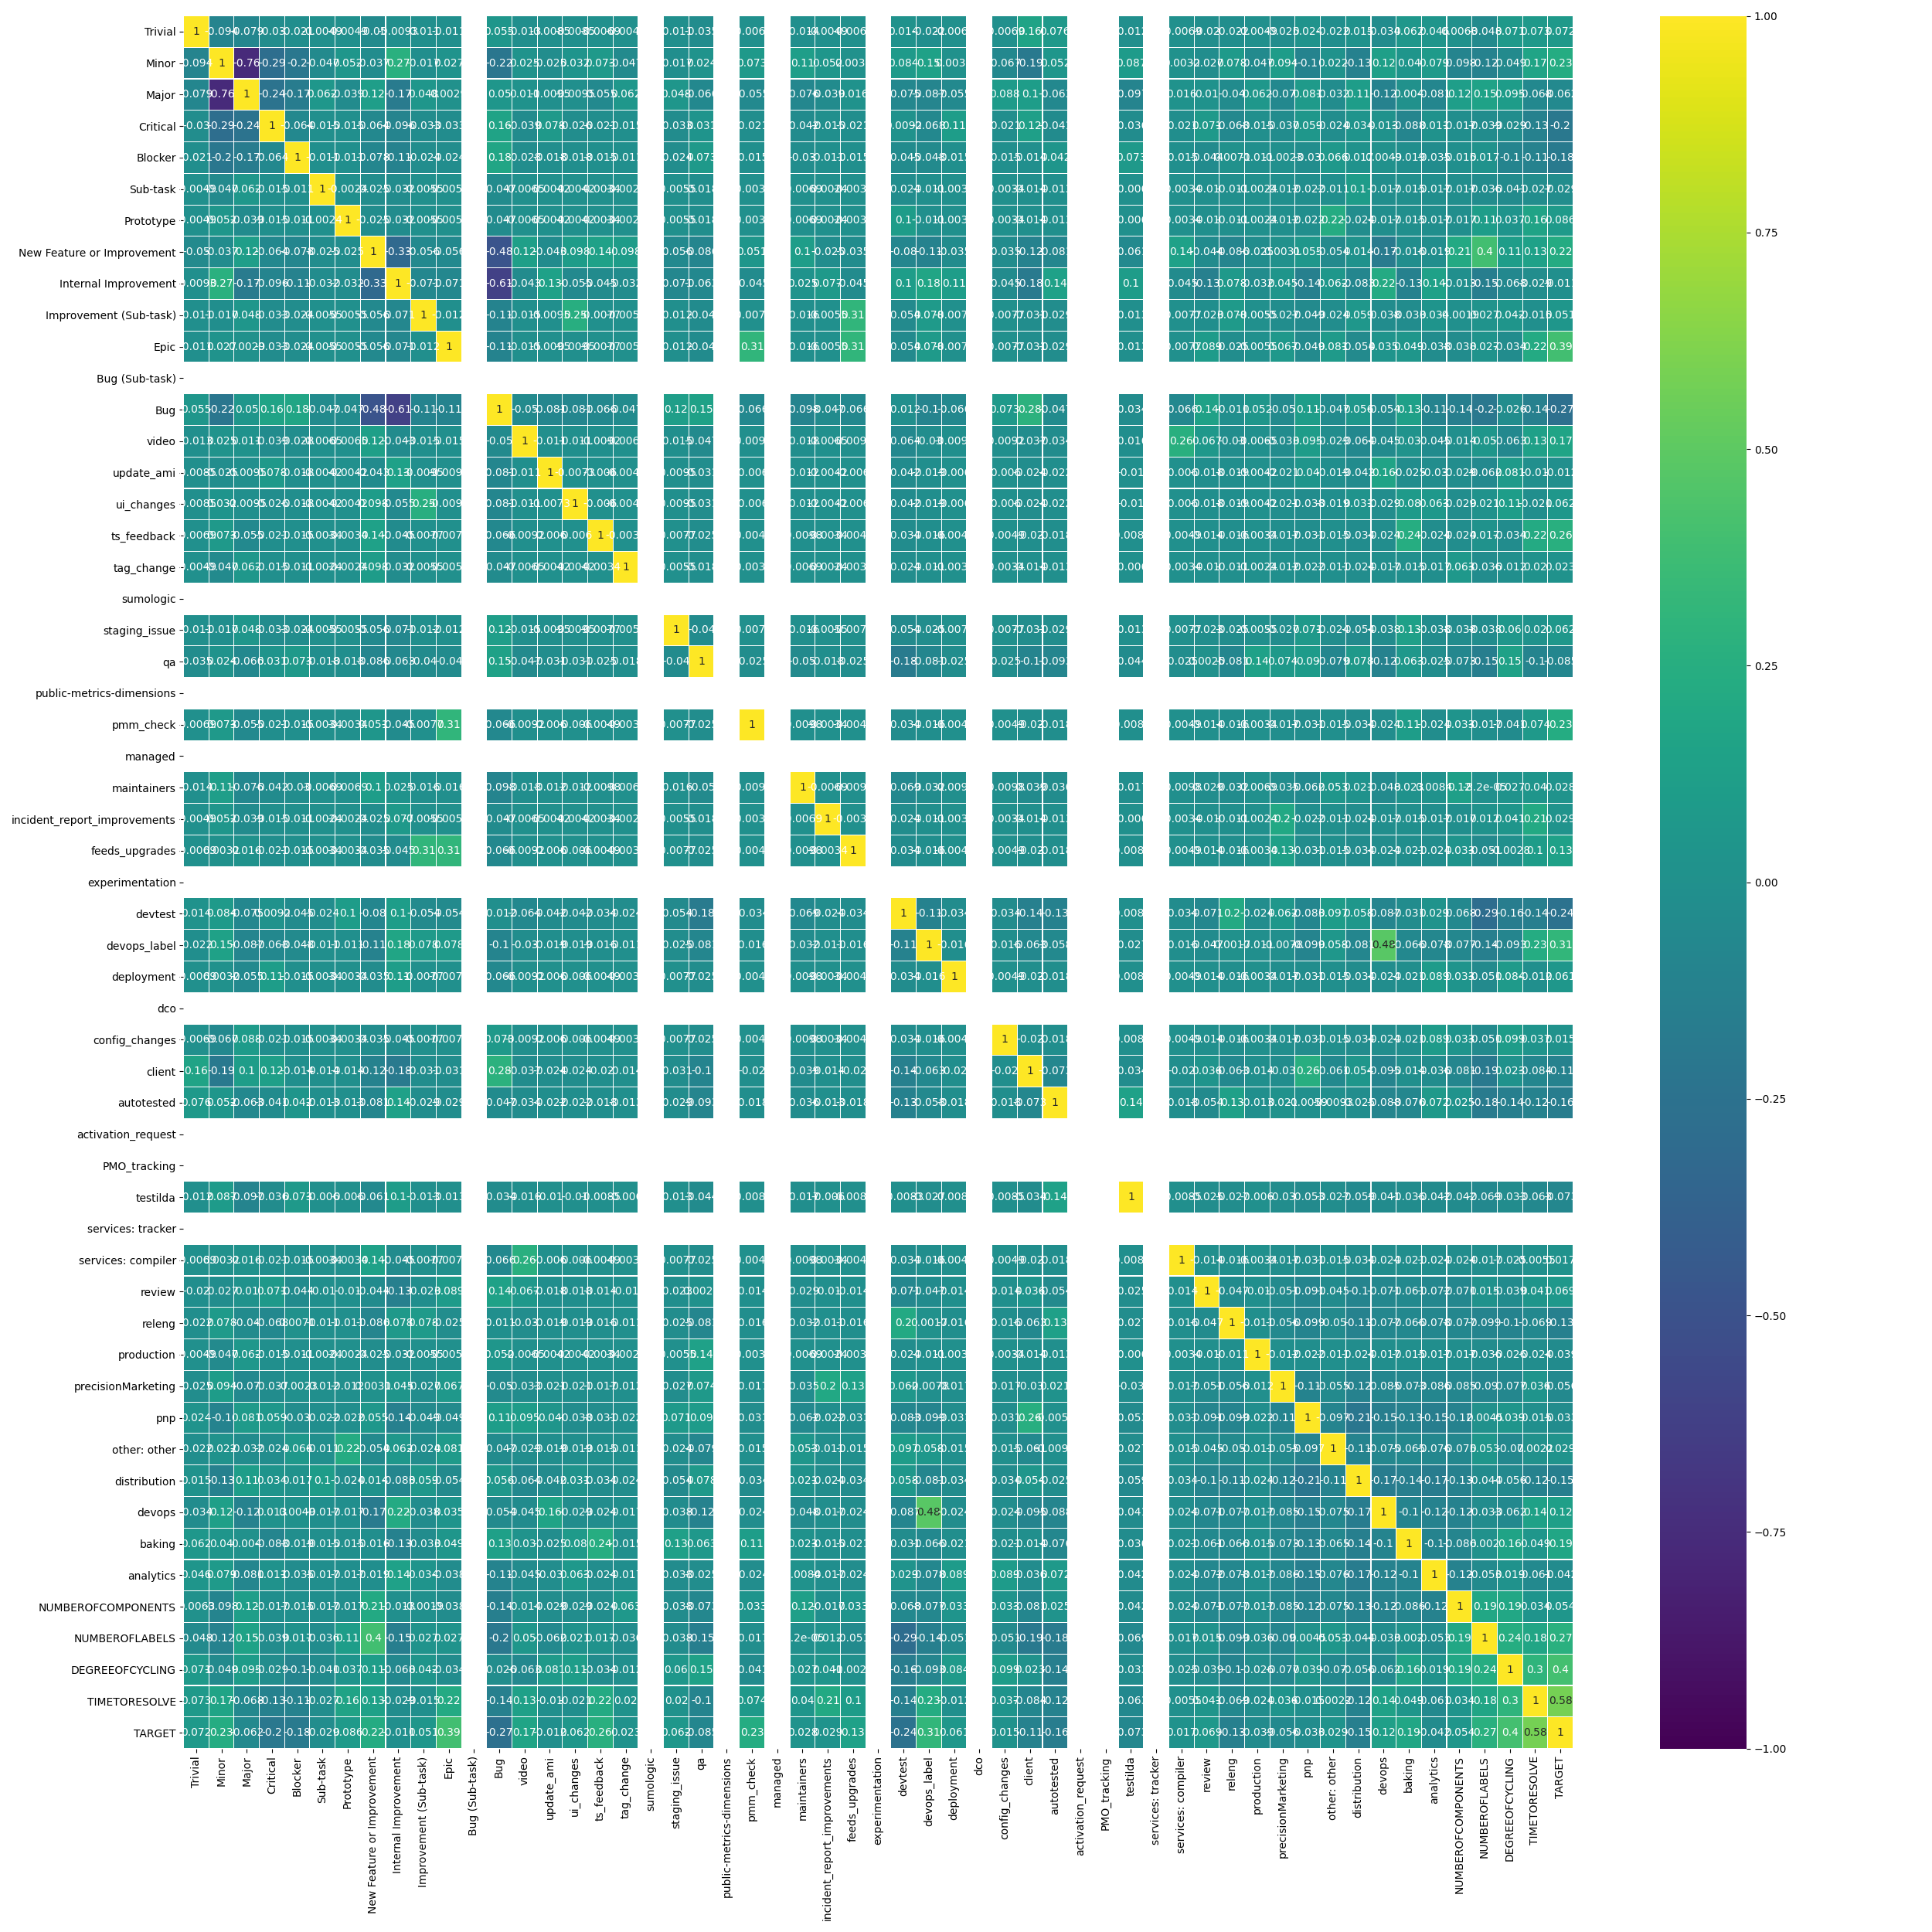
\includegraphics[width=2.5in]{feature_correlation.png}%
\label{fig_second_case}}
\caption{Simulation results for the network.}
\label{fig_sim2}
\end{figure*}

\begin{table}[!t]
	\centering
	\begin{tabular}{c|r|r|r|r}
	Statistic &  dayss & hours & hours-filtered-30 &  hours-filtered-10 \\
	\hline
	unit & days & hours & hours & hours \\
	count &  2935.000 &   2935.000 & 2771.000 & 2472.000 \\
	mean  &     8.536 &    205.252 &   95.229 &   57.273 \\
	std   &    28.265 &    678.103 &  130.036 &   59.080 \\
	min   &     0.000 &      2.000 &    2.000 &    2.000 \\
	25\%   &     1.000 &     15.000 &   13.000 &   12.000 \\
	50\%   &     2.000 &     49.000 &   44.000 &   33.000 \\
	75\%   &     6.000 &    148.000 &  121.000 &   86.000 \\
	max   &   625.000 &  15003.000 &  719.000 &  240.000 \\
	\end{tabular}
	\renewcommand{\arraystretch}{1.3}
	\caption{Dataset characteristics. }
	\label{dataset_description}
\end{table}

\begin{table}[!t]
\centering
\begin{tabular}{c|c|c|c|c}
DataSet & Method & RMSE & MAE & $R^2$ \\
\hline
\multirow{4}{*}{1}
& boost & 33.476 & 11.307 & -0.073 \\
& naive & 53.129 & 40.126 & -1.702 \\
& forest & 41.136 & 10.392 & -0.620 \\
& SVM & \textbf{33.079} & \textbf{7.988} & -0.047 \\
\hline
\multirow{4}{*}{1*}
& boost & \textbf{32.974} & 10.581 & -0.041 \\
& naive & 69.530 & 48.106 & -3.628 \\
& forest & 34.364 & 9.683 & -0.130 \\
& SVM & 33.020 & \textbf{7.961} & -0.044 \\
\hline
\multirow{4}{*}{2}
& XGBoost & 809.712 & 281.738 & -0.091 \\
& GaussianNB & 890.796 & 381.685 & -0.321 \\
& RandomForest & 1021.232 & 280.129 & -0.736 \\
& SVM & \textbf{792.962} & \textbf{193.070} & -0.046 \\
\hline
\multirow{4}{*}{2*}
& XGBoost & \textbf{792.284} & 255.451 & -0.045 \\
& GaussianNB & 941.595 & 411.579 & -0.475 \\
& RandomForest & 897.283 & 267.935 & -0.340 \\
& SVM & 792.589 & \textbf{191.877} & -0.045 \\
\hline
\multirow{4}{*}{3}
& boost & \textbf{135.966} & 89.841 & -0.026 \\
& naive & 263.943 & 209.445 & -2.865 \\
& forest & 170.992 & 103.386 & -0.622 \\
& SVM & 144.008 & \textbf{79.159} & -0.150 \\
\hline
\multirow{4}{*}{3*}
& boost & \textbf{135.020} & 90.459 & -0.011 \\
& naive & 279.474 & 232.818 & -3.333 \\
& forest & 180.686 & 113.533 & -0.811 \\
& SVM & 143.295 & \textbf{79.605} & -0.139 \\
\hline
\multirow{4}{*}{4}
& XGBoost & \textbf{54.720} & 41.941 & 0.050 \\
& GaussianNB & 122.290 & 105.834 & -3.744 \\
& RandomForest & 75.167 & 54.669 & -0.792 \\
& SVM & 59.238 & \textbf{40.390} & -0.113 \\
\hline
\multirow{4}{*}{4*}
& XGBoost & \textbf{53.706} & 42.230 & 0.085 \\
& GaussianNB & 124.868 & 109.788 & -3.946 \\
& RandomForest & 78.889 & 56.857 & -0.974 \\
& SVM & 58.114 & \textbf{39.974} & -0.071 \\
\end{tabular}
\renewcommand{\arraystretch}{1.3}
\caption{Performance of different methods on the variations of the dataset. The $*$ symbol indicates that the dataset does not contain all the initial attributes, thus it is more realistic.}
\label{table_example}
\end{table}

\bibliographystyle{IEEEtran}
\bibliography{./references}
\end{document}


